\documentclass[12pt, french]{article}

\usepackage{fancyhdr, fancybox, lastpage}
\usepackage[most]{tcolorbox}
\usepackage[a4paper, margin={0.3in, .75in}]{geometry}
\usepackage{wrapfig}
\pagestyle{fancy}
\renewcommand\headrulewidth{1pt}
\renewcommand\footrulewidth{1pt}
\fancyhf{}
\rhead{ \em{Zakaria Haouzan}}
\lhead[C]{\em{Tronc Commun scientifique - option français (TCSBiof)}}
\chead[C]{}
\rfoot[C]{}
\lfoot[R]{}
\cfoot[]{\em{Page \thepage / \pageref{LastPage}}}


\newtcolorbox{Box2}[2][
enhanced, 
    breakable,
]{
                lower separated=false,
                colback=white,
colframe=white!20!black,fonttitle=\bfseries,
colbacktitle=white!30!gray,
coltitle=black,
enhanced,
attach boxed title to top left={yshift=-0.1in,xshift=0.15in},
title=#2,#1}


\begin{document}
\begin{center}
   \shadowbox {\bf{Le Courant électrique continu }}
\end{center}
\begin{center}
   \Large{ \em{Exercices Supplémentaires}}
\end{center}

%%_________________________Exercice ! :"_________________________Exercice
   \begin{Box2}{Exercice 1 : la quantité d'électricité  }

%\begin{wrapfigure}[2]{r}{0.22\textwidth}
  %\begin{center}
	%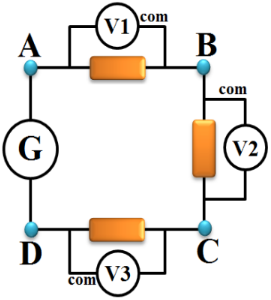
\includegraphics[width=0.22\textwidth]{./img/ex00.png}
  %\end{center}
%\end{wrapfigure}

On frotte Une baguette en ébonite avec une Fourrure de chat, et elle porte une charge électrique de
$q=-3,2.10^{-12}C$.

\begin{enumerate}
	\item  Le frottage provoque-t-elle une diminution ou une augmentation du nombre d'électrons de la
baguette?
\item Calculer le nombre de ces électrons.
\item  Calculer la charge électrique apparaissant sur la fourrure.      Avec $e =1,6.10^{-19}C$.

	\textbf{Une quantité d'électricité Q = 2,3C passe en un point d'un fil en 12 secondes.}
\item Calculer l'intensité (en mA) du courant I dans le fil.
\item  On mesure un courant de 1A dans un fil. Calculer le nombre d'électrons passant à un endroit donné
du fil en une seconde.
\end{enumerate}
   \end{Box2}


%%_________________________Exercice !2 :"_________________________Exercice
\begin{Box2}{Exercice 2 :électrisation par frottement}

   % \begin{wrapfigure}[2]{r}{0.2\textwidth}
  %\begin{center}
	  %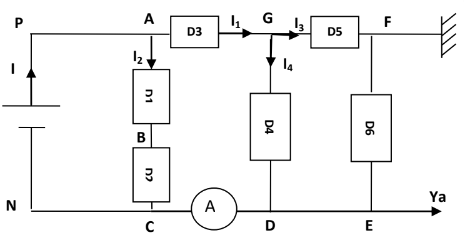
\includegraphics[width=0.2\textwidth]{./img/ex01.png}
  %\end{center}
%\end{wrapfigure}
Un bâton (A) initialement neutre, est électrisé par frottement à l’aide d’un chiffon. Sa charge
électrique devient ; $q_A = 48.10^{-18}C$.
\begin{enumerate}
	\item  Le bâton (A) a-t-il gagné ou perdu des électrons à la suite de l’électrisation ? Justifier.
	\item  Déterminer le nombre d’électrons gagnés ou perdus par (A).

		\textbf{Un deuxième bâton (B) porte une charge $q_B = 3,2. 10^{-18}C$. On met en contact l’extrémité chargée de (A)
avec l’extrémité chargée de (B).}

\item  Interpréter le phénomène qui se produit entre les deux bâtons après ce contact.
\item  Préciser, en le justifiant, le sens de transfert des électrons.

\item Déterminer le nombre d’électrons perdus par (B).
\item  Déterminer la charge de chaque bâton après le contact.
\end{enumerate}

\textbf{Données:} La charge élémentaire: $e = 1,6.10^{-19}C$.


\end{Box2}

%%_________________________Exercice ! 3:"_________________________Exercice
\begin{Box2}{Exercice 3 :intensité du courant  }
   % \begin{wrapfigure}[2]{r}{0.25\textwidth}
  %\begin{center}
	%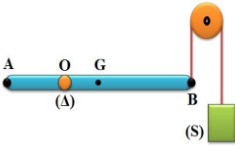
\includegraphics[width=0.25\textwidth]{./img/ex02.png}
  %\end{center}
%\end{wrapfigure}
Un courant continu a une intensité I = 0,4 A.
\begin{enumerate}
	\item  Calculer la quantité d'électricité Q débitée en 8 secondes.
	\item  Déterminer le nombre d'électrons N traversant une section du conducteur pendant ce temps.
On désire mesurer un courant de 300mA à l'aide d'un ampèremètre dont le cadran comporte 100
divisions. Les calibres de l'ampèremètre sont les suivants: 5A; 500mA; 50mA.
\item  Comment doit-on brancher l'ampèremètre dans le circuit?
\item  Quel calibre doit-on choisir; justifier la réponse.
\item Sur quelle graduation se fixera l'aiguille de l'ampèremètre?
\end{enumerate}
\end{Box2}





%%_________________________Exercice 4 : _________________________Exercice
\begin{Box2}{Exercice 4 :Utilisation d'un ampèremètre }

	\begin{wrapfigure}[1]{r}{0.28\textwidth}
		\vspace{-0.5cm}
  \begin{center}
	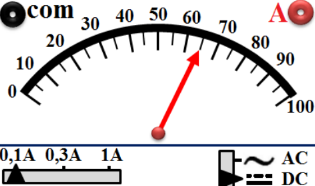
\includegraphics[width=0.28\textwidth]{./img/ex04.png}
  \end{center}
\end{wrapfigure}
La figure ci-contre représente l'image du port de l'ampèremètre.
\begin{enumerate}
	\item   Déterminer le type du courant électrique mesuré.
	\item  Déterminer le calibre utilisé.
	\item  Déterminer la valeur de l'intensité.
	\item  Calculer la quantité d'électricité traversant une section du
		circuit pendant $\Delta{t} = 10s$.
\item  Déduire le nombre d'électrons passant par cette section
pendant cette durée.
\item L'appareil est de classe 2.Déterminer la valeur de l’incertitude absolue $\Delta{I}$. Déterminer la précision de mesure.

\end{enumerate}
\end{Box2}


%%_________________________Exercice 5 : _________________________Exercice
\begin{Box2}{Exercice 5 :application de la loi des nœuds  }
   % \begin{wrapfigure}{r}{0.25\textwidth}
  %\end{wrapfigure}
	Calculer les intensités de courant manquantes dans chacun des cas suivants:
\begin{center}

	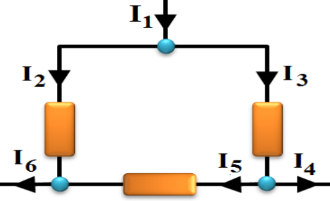
\includegraphics[width=0.25\textwidth]{./img/ex0501.png}
	\hspace{4cm}
	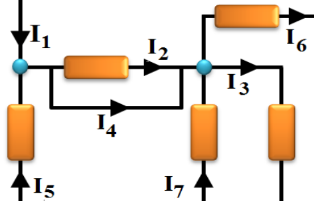
\includegraphics[width=0.25\textwidth]{./img/ex0502.png}
  \end{center}

 \hspace{2cm } $I_2=1A;$ $I_4=3A$; $I_6=2A$
 \hspace{4cm}  $I_4=7A$; $I_5=2A$; $I_6=3A$ ; $I_7=5A$
\end{Box2}
%%%_________________________Exercice 6 : _________________________Exercice

\begin{Box2}{Exercice 6 :Exploitation des circuits électriques}
\begin{wrapfigure}[2]{r}{0.28\textwidth}
		\vspace{-0.5cm}
  \begin{center}
	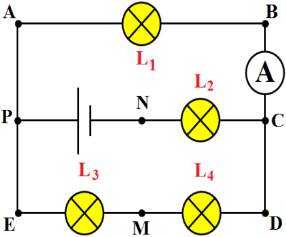
\includegraphics[width=0.28\textwidth]{./img/ex06.png}
  \end{center}
\end{wrapfigure}

On considère le circuit de la figure ci-contre, Sachant que la
quantité d’électricité Q qui traverse la section du fil AP pendant une
minute est $Q = 30 C$.
\begin{enumerate}
	\item  Calculer le nombre d’électrons qui traverse cette section pendant
\\la même durée.
\item  En déduire la valeur de l’intensité du courant $I_1$ qui traverse $L_1$.
	
\textbf{L’ampèremètre A comporte 100 divisions et possède les \\calibres
suivant : 5A ; 1A ; 300mA ; 100mA.}

\item  Quel est le calibre le plus adapté pour la mesure de l’intensité $I_1$?
\item  Devant quelle division l’aiguille de l’ampèremètre s’arrête-t-elle?
\item  L’intensité débitée par le générateur est 0,8A. Quels sont les points qui sont considérés des nœuds?

\item  Indiquer le sens du courant dans chaque branche.
\item  Déterminer les valeurs des intensités qui traversent les lampes $L_2$, $L_3$ et $L_4$.
\end{enumerate}
\end{Box2}


\begin{Box2}{Exercice 7 : Influence d'un dipôle sur la valeur de l'intensité du courant  }
	\begin{wrapfigure}[1]{r}{0.28\textwidth}
  \begin{center}
	  \vspace{-0.6cm}
	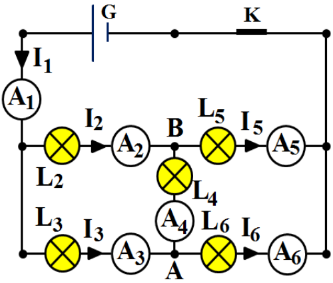
\includegraphics[width=0.28\textwidth]{./img/ex07.png}
  \end{center}
\end{wrapfigure}
Soit le circuit de la figure ci-contre où $A_1$, $A_2$, $A_3$, $A_4$, $A_5$ et $A_6$
sont des ampèremètres.
\begin{enumerate}
	\item  Les cinq lampes $L_2$, $L_3$, $L_4$ et $L_5$ sont identiques et
l’intensité\\ $I_1$ vaut $200mA$. Déterminer les valeurs des
intensités inconnues \\$I_2$, $I_3$, $I_4$, $I_5$ et $I_6$.

\item Les cinq lampes ne sont plus identiques. Les ampèremètres
$A_1$ et \\$A_2$ indiquent les intensités : $I_1=300 mA$; $I_2=100mA$ et
\\l’ampèremètre $A_4$ révèle le passage d’un courant dans le
sens A vers B et \\d’intensité $I_4=50 mA$. Déterminer les
valeurs des intensités $I_3$, $I_5$ et $I_6$.

\item Déterminer l’intensité du courant qui revient au générateur.
\end{enumerate}

\end{Box2}



\begin{Box2}{Exercice 8 : Synthèse  }
	\begin{wrapfigure}[1]{r}{0.3\textwidth}
  \begin{center}
	  \vspace{-0.6cm}
	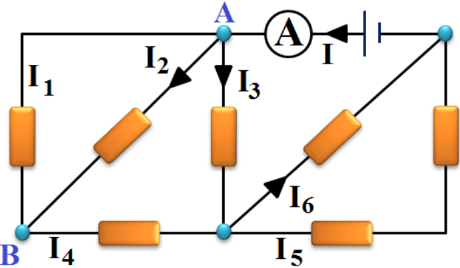
\includegraphics[width=0.3\textwidth]{./img/ex08.png}
  \end{center}
\end{wrapfigure}
Soit le circuit électrique suivant:
\begin{enumerate}
	\item Que peut-on dire des deux points A et B?
	\item  Indiquer le sens des courants manquants
dans chaque branche du \\circuit.
\item  Pour mesurer l’intensité I, on utilise un
ampèremètre à aiguille dont le calibre est
fixé à $10 A$ et son aiguille indique la
graduation 85. Calculer I.
\item En appliquant la loi des nœuds, écrire: - Une
relation entre I, $I_1$, $I_2$ et $I_3$; Une relation entre
$I_1$, $I_2$, et $I_4$; Une relation entre $I_3$, $I_4$, $I_5$ et $I_6$.
\item  Sachant que $I_2 = 2 A$, $I_3 = 3 A$ et $I_6 = 1,5 A$, calculer les intensités manquantes.
\end{enumerate}
\end{Box2}


\begin{Box2}{Exercice 9 : Synthèse  }
	Soit le circuit électrique suivant: calculer les intensités manquantes.
	%\begin{wrapfigure}[1]{r}{0.3\textwidth}
  \begin{center}
	  %\vspace{-0.6cm}
	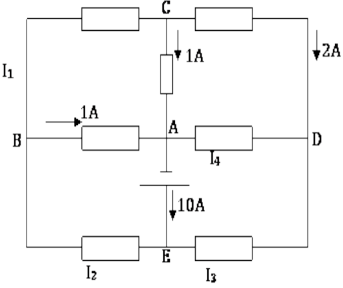
\includegraphics[width=0.35\textwidth]{./img/ex09.png}
  \end{center}
%\end{wrapfigure}


\end{Box2}



\begin{center}
	\emph{If it weren't for electricity, we'd all be watching television by candlelight.}

	\emph{\textbf{Future Is Loading...}}

\end{center}

\end{document}
